\subsection{Describe how the Stern-Gerlach experiment led to the discovery of the spin of the electron. Which properties does the spin possess?}


\paragraph{Opstillingen:} Stern-Gerlach eksperimentet, som kan ses på \cref{fig:Q08_SternGerlachEksperimentOpstilling}, blev udført af Stern og Gerlach i 1921, og skulle vise, at ... . Eksperimentet benytter en kollimeret stråle af sølvatomer, siden disse er neutralt ladede partikler, så man skulle ikke bekymre sig om en Lorentzkraft, som kunne afbøje partiklerne, i stedet for at vise, at partiklerne blev afbøjet relativit til deres formodede kvantiseret impulsmoment, hvor sidstnævnte ønskedes værende den dominerende faktor for resultatet af eksperimentet. Disse atomer blev sendt gennem et inhomogent magnetfelt skabt af en magnet, hvilket afbøjer atomerne grundet deres magnetiske dipolmoment, som skabes af deres impulsmoment, og dette danner et mønster på den fotografiske plade for enden af strålen (udenfor magneten).

\begin{figure}[!h]
    \centering
    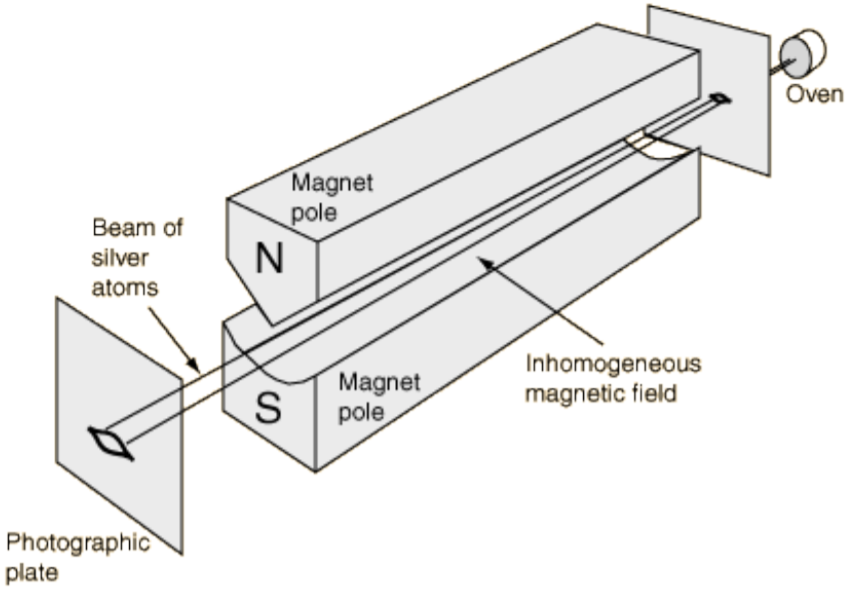
\includegraphics[width = .75\textwidth]{Q08/images/SternGerlachExperiment.PNG}
    \caption{Opstillingen af Stern-Gerlach eksperimentet.}
    \label{fig:Q08_SternGerlachEksperimentOpstilling}
\end{figure}

\paragraph{Forventning vs. resultat:} \ldots

Kigger man på forsøget med klassiske briller, så ville man forvente, at \ldots


Det blev foreslået af Uhlenbeck og Goudsmit i 1925, at elektroner havde et indre impulsmoment, også kaldet spin, hvilket viste sig at være rigtigt og kunne forklare resultatet fra Stern-Gerlach eskperimentet.

\paragraph{Egenskaber ved spin:} Spin er et impulsmoment, hvorfor det vil have de samme egenskaber som vi kender fra baneimpulsmomentet $L$:

Egenvektorerne for $\Vec{S}^2$ og $\Vec{S}_z$ vil være givet ved
\begin{align}
    \Vec{S}^2\ket{s \, m_s} &= \hbar^2 s(s+1) \ket{s \, m_s} \label{eq:Q08_EgenvektorligningForS^2} \: , \\
    \Vec{S}_z\ket{s \, m_s} &= \hbar m_s \ket{s \, m_s} \label{eq:Q08_EgenvektorligningForS_z}
\end{align}